\documentclass[oneside,a4paper,12pt]{book}
\usepackage[english]{babel}
\usepackage[utf8]{inputenc}
\usepackage{microtype}
\usepackage{graphicx}
\usepackage{qtree}
\usepackage{amsmath}
\usepackage{float}
\usepackage{blindtext}
\usepackage{amsthm}
\usepackage{soul}
\usepackage{amssymb}
\usepackage{placeins}
%%Programming packages
\usepackage{program}
%%\usepackage[section]{algorithm} % Bullshit error
\usepackage{algorithm} % Bullshit error


%%\usepackage{algorithmic}
%\usepackage{algorithmicx}
\usepackage{algpseudocode}
\usepackage{float}
\usepackage{listings}
%%\usepackage{algorithm2e}
%%end programming
\usepackage{verbatim}
\usepackage{proof}
\usepackage{fitch}

\usepackage{booktabs}
\usepackage{fancyhdr}
\usepackage[a4paper, inner=1.5cm, outer=1.5cm, top=2cm, bottom=3cm, bindingoffset=0cm]{geometry}
\fancyhf{}
\fancyhead[LE,LO]{\leftmark}
\fancyhead[RE,RO]{\nouppercase{\rightmark}}
%\fancyfoot[LE,RO]{\thepage}
\pagestyle{fancy}
\cfoot{Lazuli \thepage}
\lfoot{}
\restylefloat{algorithm}
\setcounter{tocdepth}{1}
\usepackage[hidelinks, linktoc=all]{hyperref}

\usepackage[utf8]{inputenc}

% Default fixed font does not support bold face
\DeclareFixedFont{\ttb}{T1}{txtt}{bx}{n}{12} % for bold
\DeclareFixedFont{\ttm}{T1}{txtt}{m}{n}{12}  % for normal

% Custom colors
\usepackage{color}
\definecolor{deepblue}{rgb}{0,0,0.5}
\definecolor{deepred}{rgb}{0.6,0,0}
\definecolor{deepgreen}{rgb}{0,0.5,0}



% Python style for highlighting
\newcommand\pythonstyle{\lstset{
language=Python,
basicstyle=\ttm,
otherkeywords={self},             % Add keywords here
keywordstyle=\ttb\color{deepblue},
emph={MyClass,__init__},          % Custom highlighting
emphstyle=\ttb\color{deepred},    % Custom highlighting style
stringstyle=\color{deepgreen},
frame=tb,                         % Any extra options here
showstringspaces=false            % 
}}


% Python environment
\lstnewenvironment{python}[1][]
{
\pythonstyle
\lstset{#1}
}
{}

% Python for external files
\newcommand\pythonexternal[2][]{{
\pythonstyle
\lstinputlisting[#1]{#2}}}

% Python for inline
\newcommand\pythoninline[1]{{\pythonstyle\lstinline!#1!}}

\usepackage{multicol}
\begin{document}
\begin{titlepage}
\center
\hrule \hfill \\
{\Large Analyzing Factors Affecting POLYITAN-1 Telemetry Demodulation\\[.1in]}
\hrule 

\vspace{1in}
\begin{figure}[h]
    \centering
    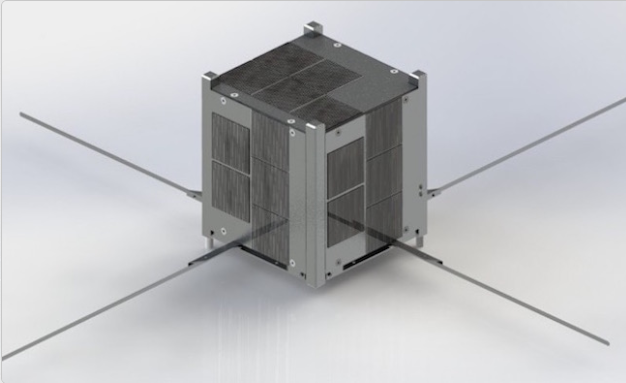
\includegraphics[width=0.8\textwidth]{images/Selection_837.png}
    \caption{\small\textit{The POLYITAN-1 satellite as it would be deployed on orbit\cite{kpi}}}
    \label{fig:Selection_837.png}
\end{figure}

\vspace{2in}

{\Large Ada Lazuli\\[.2in]}
{  ajl6952@psu.edu\\[.3in]}

{\itshape \today}
\end{titlepage}
\include{conventions}
\frontmatter
\mainmatter

\subsection*{Introduction}
\hspace{\parindent} POLYITAN-1 is a Ukrainian cube satellite that was placed into orbit in 2014 as a technology demonstration satellite\cite{celes}. The satellite network of ground stations (SatNOGS) is a community of amateur radio operators with hundreds of satellite ground stations and has made approximately 11,000 attempts at demodulating radio signals from POLYITAN-1. However, the community has only achieved a success rate of 47.55\%\cite{satnogsnetwork}. At this point in time, it is unclear as to why the community is having such a difficult time demodulating radio signals from this satellite. 

It is likely that the elevation angle (that is, the degrees off the horizon from the perspective of the observer), whether the satellite is illuminated, since illumination means the satellite should have an abundance of power for transmission, and whether the observer is being illuminated due to increased atmospheric interference and receiver thermal noise are key factors that affect whether the radio signal is demodulated. An observation study will be conducted to assess whether transmission rate is highest when the elevation angle is high, the satellite is illuminated, and the ground station is not illuminated.

\section*{The Data }
\hspace{\parindent} The SatNOGS community makes their data available under the creative commons license and stipulates that credit must be given for the data source and does not place any other restrictions on the data use\cite{satnogs}.  A python script was used to pull approximately 15,000 observations from the SatNOGS website. Then, to enrich the data,  the python skyfield package was used to determine the highest elevation in a given pass, whether the satellite was illuminated by the sun during the pass, and whether the ground station was illuminated by the sun during the pass\cite{skyfield}. 

\begin{figure}[h]
    \centering
    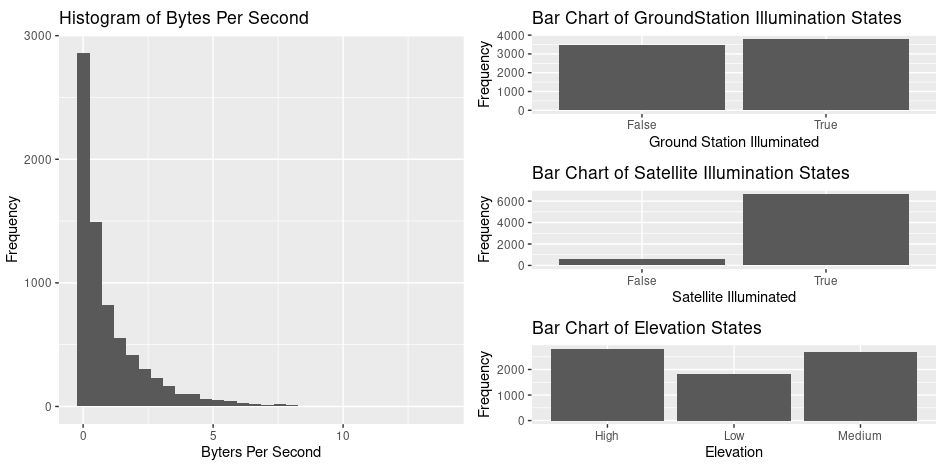
\includegraphics[width=0.8\textwidth]{images/Selection_905.png}
    \caption{\small\textit{Plot depicting a histogram of the data collected by various ground-stations, as well as, the number of each qualitative variable class}}
    \label{fig:Selection_905.png}
\end{figure}

This is specifically how the data will be referred as the following during the study:

\begin{description}
\item[Response]: The transmission speed in bytes per second.
\item[Factor A]: Elevation Angle,  levels: Low, Medium High
\item[Factor B]: Satellite Illumination State,  levels: True, False
\item[Factor C]:Receiver Illumination State  levels: True, False
\end{description}

Additionally, as seen in Figure \ref{fig:Selection_905.png}, the data has strong right skew that will need to be transformed to ensure all assumptions of the model are met. Additionally, the collected data has strong class imbalance where very few of the observations have the satellite in darkness.

\section*{Method}
\hspace{\parindent} To control for the variation between the various ground station hardware and interference environments, the ground station ID will be utilized as a blocking factor. The intention is to implement Randomized Complete Block Design (RCBD). However, if the data is too sparse, then a switch to Completely Randomized Design (CRD) will happen. Assuming there is sufficient data for RCBD, the model used for this study shall be:

$$
Y_{ijklm} = \mu  + \alpha_i + \beta_j  + \gamma_k + \delta_l + (\alpha\beta)_{ij} + (\alpha\gamma)_{ik} + (\beta\gamma)_{jk} + (\alpha\beta\gamma)_{ijk}  + \epsilon_{ijklm}
$$

Where:

\begin{itemize}
\item $\mu$ is the mean quantity of data demodulated,
\item $\alpha_i$ is fixed effect of the elevation angle
\item  $\beta_j$ is the fixed effect of the satellite illumination state
\item $\gamma_k$ is the fixed effect of the ground station illumination state
\item $\delta_l\overset{iid}{\sim} N(0, \sigma^2_\delta)$ is the random error associated with the the ground station block.
\item $(\alpha\beta)_{ij}$, $ (\alpha\gamma)_{ik}$ , $(\beta\gamma)_{jk}$,  and $ (\alpha\beta\gamma)_{ijk} $ are the interaction effects between the elevation angle, the satellite illumination, and the ground station illumination.
\item $\epsilon_{ijklm} \overset{iid}{\sim} N(0, \sigma^2_\epsilon)$ is the random error associated with the observation.
\end{itemize}

\section*{Results }

It became clear early in the analysis that additional steps needed to be taken to prepare the data. To implement RCBD, the data was subsetted such that only observations from stations were kept only if the station appeared more than 10 times in the data. This led to the data consisting of 14829 observations from 77 ground-stations. Additionally,  the transmission rate needed to undergo transformation to meet the assumptions of ANOVA, as evidenced by  Figure \ref{fig:Selection_888.png} of the appendix. The box-cox method was used in SAS to find a $\lambda$ value of zero (depicted in  Figure \ref{fig:Selection_887.png}), suggesting that the transmission rate should be transformed by taking the logarithm. 

Following this transformation, the Q-Q plot is significantly healthier and the ``megaphone'' affect is drastically reduced,  as seen in \ref{fig:Selection_887.png}. The residuals versus fits plot has a band of approximately 3.5 on the top but has a line with a negative slope along the bottom. While this is a violation of the assumption of equal variance, this ANOVA study consists of 14829 observations and the conclusions should still be relevant despite the slight violation.

\begin{figure}[H]
    \centering
    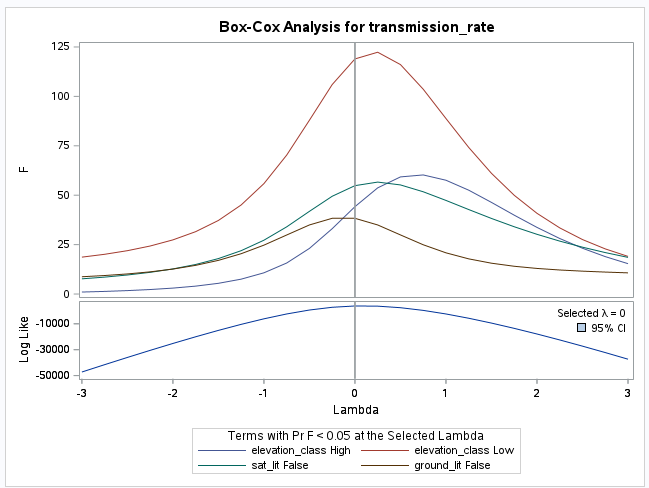
\includegraphics[width=0.5\textwidth]{images/Selection_887.png}
    \caption{\small\textit{Using the box-cox method in SAS to discover a $\lambda$ value of 0 suggesting a logarithmic transformation.}}
    \label{fig:Selection_887.png}
\end{figure}

\begin{figure}[H]
    \centering
    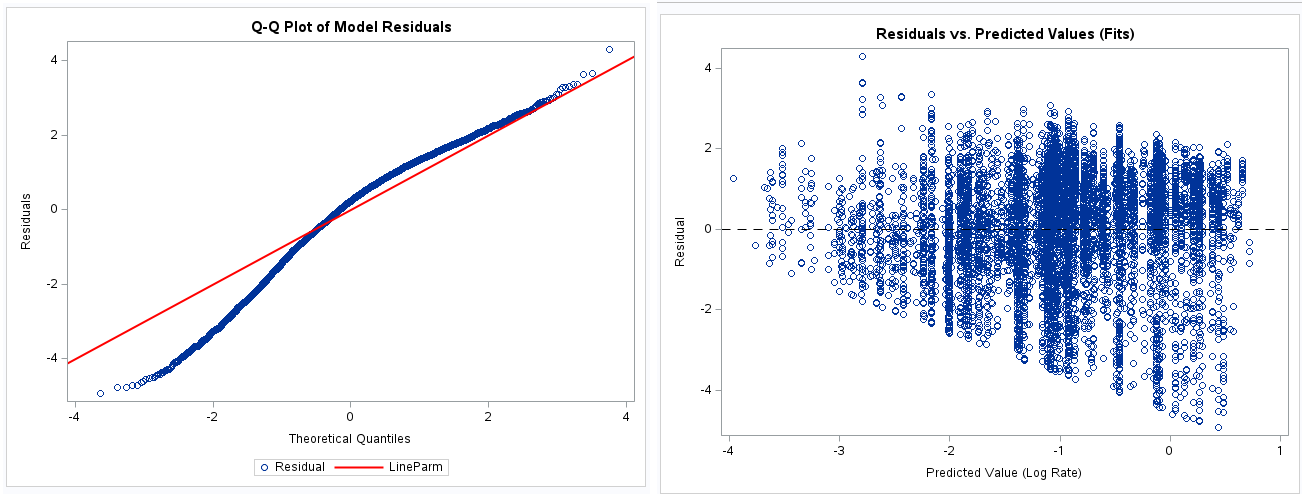
\includegraphics[width=0.8\textwidth]{images/Selection_889.png}
    \caption{\small\textit{Q-Q Plot and Residuals vs Fits plots with the transformed transmission rate, showing significant improvements}}
    \label{fig:Selection_889.png}
\end{figure}

Figure \ref{fig:Selection_890.png}  of the appendix captures the full ANOVA table and revealed a problem with the collected data. Due to the satellite's low orbit, most of the observations had matching satellite illumination and ground-station illumination, resulting in very significant col-linearity. This also explains why the Sum of Squares were very similar for the both terms. Due to the col-linearity, the decision was made to reduce the model by dropping the satellite illumination variable. The reduced model ANOVA table is captured in  figure \ref{fig:Selection_891.png} and the updated model with the same indices established earlier is:

\begin{figure}[H]
    \centering
    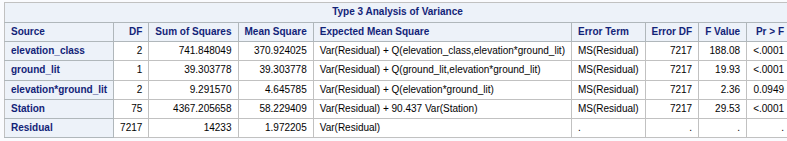
\includegraphics[width=0.99\textwidth]{images/Selection_891.png}
    \caption{\small\textit{Updated ANOVA table without the co-linearity using the updated model.}}
    \label{fig:Selection_891.png}
\end{figure}

$$
Y_{iklm} = \mu  + \alpha_i  + \gamma_k + \delta_l  + (\alpha\gamma)_{ik}  + \epsilon_{iklm} 
$$

\subsubsection*{Evaluating $\alpha_i $}

The coefficient $\alpha_i $ represents the fixed effect of the elevation angle and was found to differ meaningfully from zero:
$$
\begin{aligned}
&H_0: \forall_i  [\alpha_i = 0] ; \quad H_a:  \exists_i  [\alpha_i \neq 0]\\
&F^* = \frac{370.924}{1.972} = 188.1\\
\end{aligned}
$$
The p-value of  $F_{2,7217} 188.1 < 0.001$, therefore reject the null hypothesis. Figure \ref{fig:Selection_900.png} of the appendix captures the diffogram and tukey means groupings, showing that high elevation observations have the highest transmission rates while low elevation observations have the lowest transmission.

\subsubsection*{Evaluating $\gamma_k $}

The coefficient $\gamma_i $ represents the fixed effect of the ground-station illumination and was found to differ meaningfully from zero:
$$
\begin{aligned}
&H_0: \forall_k  [\gamma_k = 0]; \quad H_a:  \exists_k [ \gamma_k \neq 0]\\
&F^* = \frac{39.30}{1.972} = 19.93\\
\end{aligned}
$$
The p-value of  $F_{1,7217} 19.93 < 0.001$, therefore reject the null hypothesis.  Figure \ref{fig:Selection_901.png} of the appendix captures the diffogram and tukey means groupings for ground illumination, the transmission rate is higher in darkness.

\subsubsection*{Evaluating $(\alpha\gamma)_{ik} $}

The coefficient $(\alpha\gamma)_{ik} $ represents the interaction effect of the elevation angle and the ground-station illumination and was not found to differ meaningfully from zero.
$$
\begin{aligned}
&H_0: \forall_{i,k}  [(\alpha\gamma)_{ik} = 0]; \quad H_a:  \exists_{i,k}  [(\alpha\gamma)_{ik} \neq 0]\\
&F^* = \frac{4.646}{1.972} = 2.36\\
\end{aligned}
$$
The p-value of  $F_{2,7217} 2.36 \approx 0.0949$, therefore fail reject the null hypothesis.


\section*{Conclusion }

In conclusion, it was discovered that the elevation angle of the ground-station relative to POLYITAN-1 and whether the ground-station is illuminated have a significant effect on the demodulation of radio signals from the satellite. This conclusion is reasonable as higher elevation passes would have less obstruction from objects, such as trees or buildings. Additionally, the finding higher transmission rates is reasonable due to less interference in the atmosphere and thermal noise on the receiver from the sun. It follows from these observations that the SatNOGS community could achieve better performance for POLYITAN-1 telemetry demodulation by scheduling only for high elevation passes at night. Moreover, due to the representation of the collected data, this study was limited to effects of the transmission environment and not on the satellite itself. This study was also unable to explore the likelihood of demodulating a signal and was restricted to the quality of the demodulation using the transfer rate. Future work could focus on the satellite itself by collecting data over a larger period and restricting observations to only high elevation night time passes study the few occurrences when the satellite is illuminated while the ground-station is not. If such a study concluded that there was a difference in transmission rate then that could be indicative of a problem with the satellite's power subsystem, such as the onboard batteries.


\pagebreak

\section*{Appendix}

\begin{figure}[h]
    \centering
    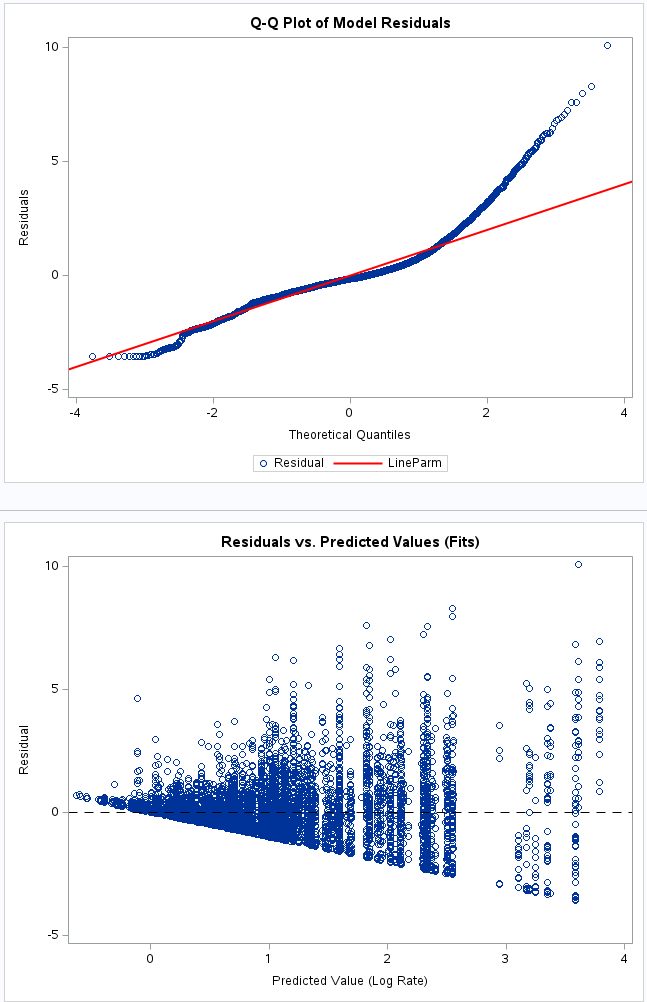
\includegraphics[width=0.5\textwidth]{images/Selection_888.png}
    \caption{\small\textit{Q-Q Plot and Residuals vs Fits plots showing significant violations of normalcy and constant variation of the non-transformed transmission rate.}}
    \label{fig:Selection_888.png}
\end{figure}

\begin{figure}[h]
    \centering
    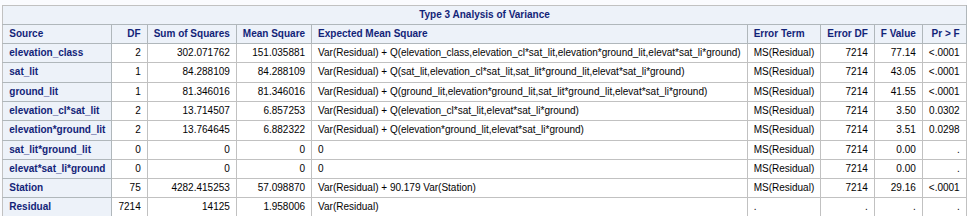
\includegraphics[width=0.99\textwidth]{images/Selection_890.png}
   \caption{\small\textit{ANOVA table showing significant co-linearity between satellite illumination and ground-station illumination.}}
    \label{fig:Selection_890.png}
\end{figure}

\begin{figure}[h]
    \centering
    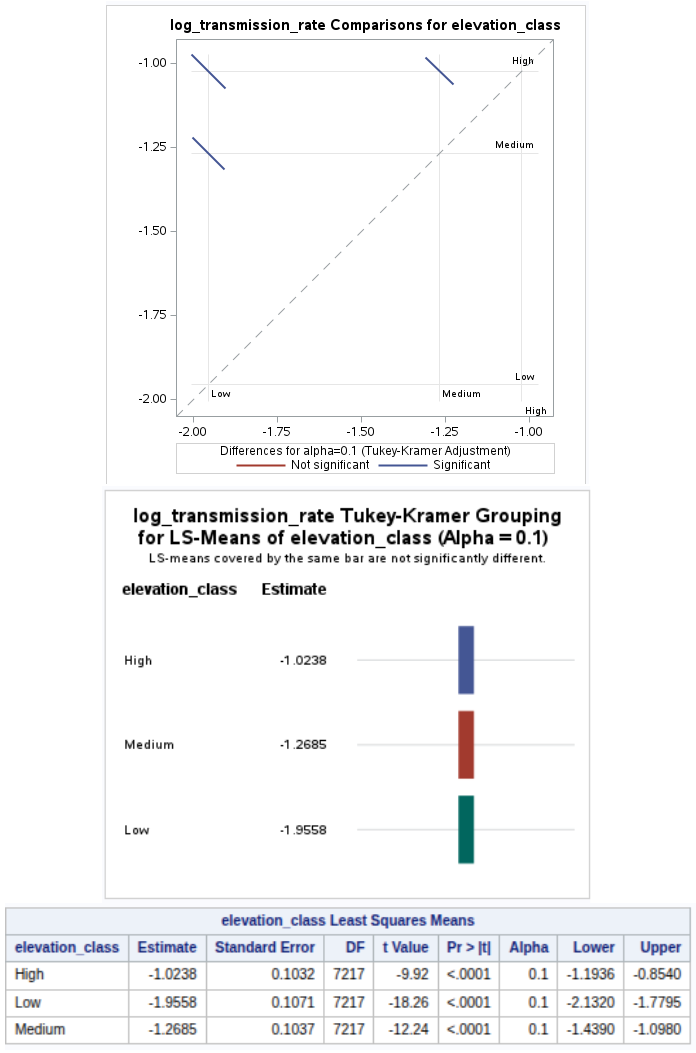
\includegraphics[width=0.59\textwidth]{images/Selection_900.png}
   \caption{\small\textit{Diffogram and tukey grouping for elevation levels}}
    \label{fig:Selection_900.png}
\end{figure}

\begin{figure}[h]
    \centering
    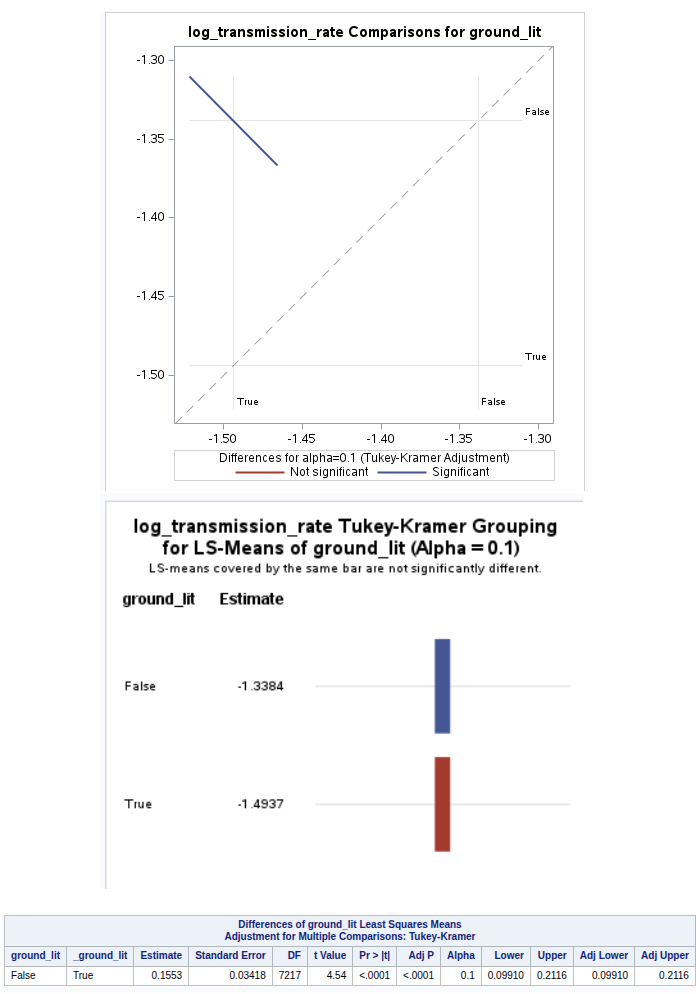
\includegraphics[width=0.59\textwidth]{images/Selection_901.png}
   \caption{\small\textit{Diffogram and tukey grouping for ground illumination levels}}
    \label{fig:Selection_901.png}
\end{figure}

\begin{thebibliography}{7}

\bibitem{kpi}
KPI Research Laboratory. (2015). \textit{PolyITAN-1}. Retrieved April 13, 2026 from http://www.cubesat.org.ua/en/nano-satellites/polyitan-1

\bibitem{celes}
Kelso, T. (2026). \textit{SATCAT Results for 40042}. Retrieved April 13, 2026 from https://celestrak.org/satcat/table-satcat.php?CATNR=40042\&PAYLOAD=1\&MAX=500

\bibitem{skyfield}
Rhodes, B. (2026). \textit{Skyfield: Elegant Astronomy for Python}.   Retrieved April 13, 2026 from https://rhodesmill.org/skyfield/

\bibitem{satnogs}
SatNOGS Community. (2026). \textit{About: SatNOGS Network}. Retrieved April 13, 2026, from https://network.satnogs.org/about/

\bibitem{satnogsnetwork}
SatNOGS Network. (2026). \textit{POLYITAN-1 Observations}. Retrieved April 13, 2026, from https://network.satnogs.org/observations/?sat\_id=UIYC-4491-1380-9406-8215

Observations from the SATNOGS network used in this study were provided by:

\begin{multicols}{3}
\tiny
\begin{itemize}
    \item 431 - PE0SAT-11
    \item 2173 - PE0SAT-21
    \item 1466 - PE0SAT-12
    \item 1696 - PE0SAT-31
    \item 2968 - UX5UL
    \item 3523 - IK1JNS-UHF
    \item 766 - Dunchurch
    \item 3538 - PU4ELT
    \item 2012 - SP7THR-UHF
    \item 1710 - EU1AEM
    \item 2029 - EU1AEM
    \item 91 - M0EYT / 2E0NOG
    \item 2729 - YL3GBC
    \item 1864 - SA2KNG Omni UHF/VHF
    \item 1936 - VK4JBE-UHF
    \item 71 - PV8DX
    \item 3122 - Lovets
    \item 812 - PF\_DE\_UHF\_X\_DIPOLE
    \item 1861 - LW2DYB
    \item 2015 - Drachten
    \item 2410 - GAO UHF
    \item 2617 - K2PI
    \item 1376 - Venables\_Shed\_UHF
    \item 1416 - PE2BZ-437
    \item 3369 - EST VENUS
    \item 3746 - SatNOGS\_Pecna\_1\_UHF
    \item 2134 - MAUSyagi
    \item 1675 - MAUSyagi
    \item 3762 - F4TNK-UHF
    \item 6 - Apomahon
    \item 3387 - YO4DFT- S + L band
    \item 2934 - UFS-GS
    \item 2510 - MAUSyagi
    \item 2987 - VU2JEK\_Nitin
    \item 754 - W6MSU UHF
    \item 1155 - ArgusNavis
    \item 3600 - YO4DFT az 315 degrees -North West
    \item 2739 - SV5QNF - VHF
    \item 3590 - EuroSpaceHub-UCM
    \item 3106 - DEX-ONE
    \item 3918 - YL3CT-1
    \item 2394 - YC7OIZ
    \item 3951 - UT4UYF/M
    \item 3905 - LW1EXU-GroundStation
    \item 1533 - SV5QNF - UHF
    \item 2247 - Mainz435
    \item 3925 - UT4UYF/P
    \item 4188 - ISAE.Supaero UHF
    \item 2125 - M0GLU
    \item 3508 - KEREL-UHF-RLP
    \item 3855 - GS ChNord UHF
    \item 3963 - NWLGS1
    \item 3117 - RA3PPY
    \item 4372 - IK3SVW-1
    \item 3020 - Jim UHF
    \item 4151 - DEX-X
    \item 2416 - N5ZKK-UHF-HELICAL
    \item 1860 - BEEGND-4
    \item 4460 - Sofia SAT Club - Bay Ivan
    \item 4111 - Plyachka
    \item 4356 - KsiezeMale
    \item 1167 - F1SXJ
    \item 3763 - plat0-3a
    \item 1002 - M0ZJO Station \#1
    \item 4497 - VA3HEV
    \item 4451 - I LOVE BALI YES
    \item 40 - CGBSAT-UHF
    \item 4595 - EA4TA
    \item 4391 - UHF-VHF Sofia City Balcony
    \item 3438 - StreetDirt UHF
    \item 1565 - Dumbravita - VHF/UHF - YO2MKE
    \item 1597 - YB8XM
    \item 1672 - AAS Ager Carballada
    \item 1523 - UHF Essendon
    \item 980 - PF\_DE\_UHF\_Yagi
    \item 1667 - AAS Berga Carballada
\end{itemize}
\end{multicols}

\end{thebibliography}


\end{document}
